\section{普通話會取代粵語成為香港的主流語言嗎?}
\label{sec:sec13}

按目前趨勢,中短期內不會。不過儘管廣州話目前尚處於主導地位,香港人對語言和文字近年已變得十分敏感。畢境語言是身分認同的重要元素,前文提到七十年代廣東流行曲的興起對香港認同的出現有舉足輕重的作用(見\hyperref[sec:sec5]{問題五})。此外,普通話的流行程度也被一些輿論視為中國大陸來港移民人數的指標,認為普通話越流行就代表土生土長的香港人在比例上變少,而大陸移民則拒絕融入本地文化,要守護香港人的獨特身分將會變得困難。

從人口普查的統計數據去看,廣州話在香港仍然十分普遍,是88.9\%香港居民的慣用語言(即在家中使用的語言),而能說廣東話的更達94.6\%,只有5.4\%的香港人不會。除了廣州話外,以慣用語言算香港的主要語言尚有英語(4.3\%)、普通話(1.9\%)、福建話(1.0\%)和客家話(0.7\%),另有其他少數族裔語言如日本語、泰語和南亞語系等。近年廣州話作為慣用語言的比例有輕微下降,而普通話的則有輕微上升,但說到普通話要成為香港的主流語言,數據上暫時看不出來。

至於輿論對中國大陸移民的擔憂,數據上也未能證實。以華人計算,來港不足一年的華人當中能說廣東話的比例為74.6\%,來港一至三年的為86.6\%,來港四至六年的為95.8\%,來港7-10年的為97.2\%,來港十年或以上的為99.1\%。換言之,不懂得廣州話的外來華人人口要不是後來學會了,就是離開了,語言上的影響未如輿論擔憂般強烈。另有統計顯示雖然近年從中國大陸來港的新移民當中,慣用語言不是廣州話的越來越多,但能使用廣州話交談的比例卻未見明顯下跌。也就是說,他們來港後出於日常溝通等生活需要,絕大多數還是學會了廣州話。

\begin{figure}[htbp]
    \centering
    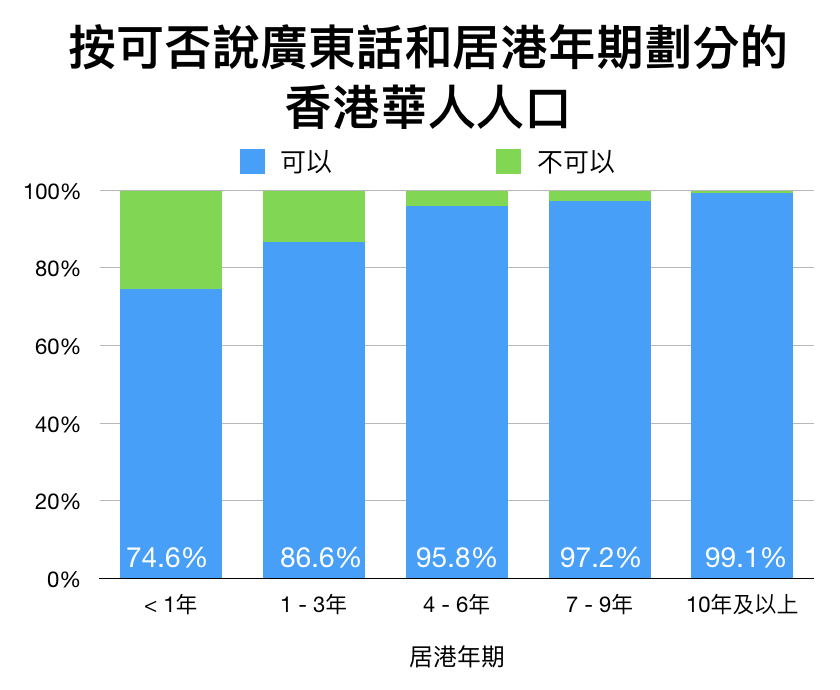
\includegraphics[width=0.7\textwidth]{c13/h-klesson1-019.png}
    \caption{華人能說廣東話的比例按居港年期上升} 
\end{figure}

當然,上述的只是普遍情況,個別場合的語言環境可以有更明顯的改變。例如一些和中國大陸有大量業務往來的企業,往往會招聘不少大陸專才或在港畢業的大陸留學生工作,職場語言就會變成普通話。此外,由於上述數據只計算香港居民,不計算遊客,所以不能反映出在某些服務中國大陸遊客為主的場所,普通話已變成該處的主要交談語言。

那麼香港人口當中懂得普通話的比例又如何?同樣只計算華人人口,二零零六年時能說普通話的比例是41.8\%,到了二零一六年已升至51.8\%。這改變相信來自中港交流頻繁,出於工作需要很多人都自己學會了普通話;政府在普通話教育方面的投放,也帶來明顯影響。

不過普通話教育應如何推行,民間有不同意見,當中有兩條問題至關重要。第一,學習普通話應該出於自願,還是該強制執行?第二,學習普通話應該和使用廣州話分開進行,還是要取代廣州話的教學地位?近年香港出現強制學習普通話,以及普通話取代廣州話教學地位的趨勢,使得不少輿論認為普通話取代廣州話已成官方政策,最終會演變為文化侵略,香港下一代將會不再重視甚至不懂得廣州話。不少輿論擔憂上海話在上海新一代之間不再流行的情況,將會在香港重演。

強迫學習普通話的問題,在香港浸會大學普通話豁免試風波中最為明顯。浸大自二零零八年前起要求學生必須修讀帶學分之普通話課程,考試合格方可畢業。有學生認為要求不合理,於是浸大於二零一七年起推出測試,合格者可豁免修讀普通話課程。結果測試只有三成學生合格,學生質疑測試標準有問題,甚至認為語文中心刻意降低合格率來保障自己的生源。事件在校內激化為示威衝突,在校外則演變成大學語文政策之爭。大學認為學習普通話對學生有利,可以用各種方式鼓勵自願學習;但將之變成畢業的要求,和大學本身作為思想自由堡壘的角色有否衝突,成為關注焦點。

中小學教育方面,爭議則在於廣州話的教學地位會否被普通話取代。香港政府於二零零八年起推出《協助香港中、小學推行「以普通話教授中國語文科」計劃》,也就是「普教中」。政府推動以普通話取代廣州話作為中文課的教學語言,理據一方面是要統一「聽、說、讀、寫」,減少香港或廣東俚語入文的情況;另一方面則可加強普通話學習,有利日後跨境交流。不過,有作家和研究語文的學者指出,不一定要用普通話學習才能學好寫作,強行使用卻會阻礙師生溝通。有成績評估機構的調查發現,「普教中」學生的閱讀水平反過來比非「普教中」學生低。政府在推動此政策十年以來,仍未能提供數據支持其實際成效。

\begin{figure}[htbp]
    \centering
    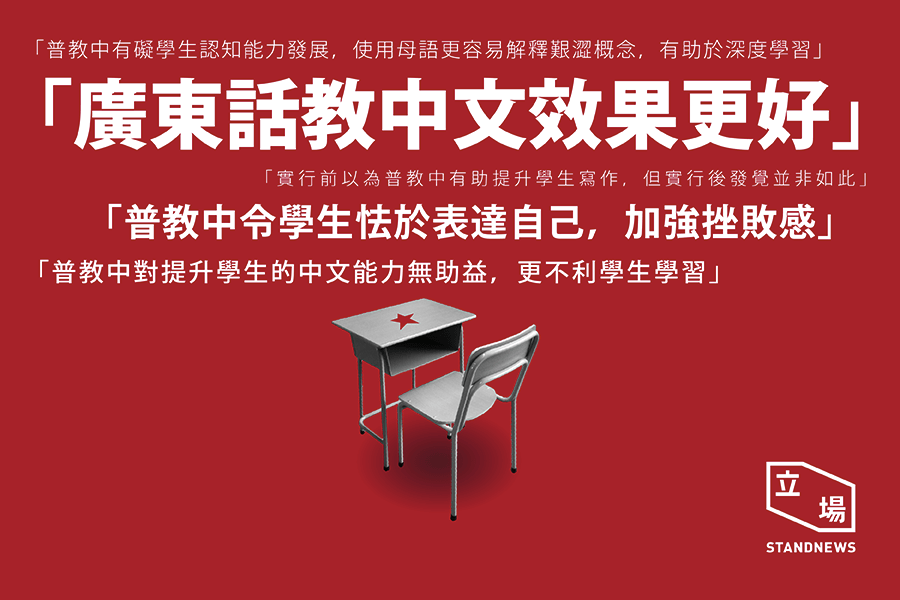
\includegraphics[width=0.7\textwidth]{c13/h-klesson1-020.png}
    \caption{普教中的成效引起很大爭議} 
\end{figure}

除了廣州話和普通話之爭外,類似的爭端也在書寫系統和字詞應用出現。書寫系統之爭,在於繁體字和簡體字在香港的地位。簡體字的使用對持本土觀點者來說,也代表來自中國大陸的文化入侵。他們往往會把繁體字稱之為正體字,強調其為正字本源;再激進一點的,會把簡體字稱為「殘體字」,並嘲笑他們眼中簡體字的弱點(如同字多義更常出現,引發「後后不分」等問題)。

字詞應用方面,也有持本土觀點者認為要守護香港身份,就要嚴格拒絕一些源於中國大陸的流行字詞。例如一段婚姻當中出現女性第三者,香港過去的說法是將該女性稱為「二奶」,近年則開始通用中國大陸流行的「小三」,引發不少持本土觀點者的不滿,甚至稱之為「匪語」。曾有餐廳為了服務中國大陸旅客,在餐牌上把香港通用的「沙律」寫成「沙拉」,亦引發輿論強列不滿。不過,甚麼是所謂的「匪語」,甚麼才不是,有時也不易回答。例如「質素」和「素質」的分別,不少持本土觀點者強調香港人不應遷就中國大陸的「素質」說法,有語言學者研究後則發現兩者背後原來有相當複雜的歷史和當代含義,不易釐清。類似案例點出了一個問題:文化議題往往很難非黑即白,但政治議題卻常常強調立場明確,兩者之間的落差難免會帶來各種爭端誤解。近年就有常常出現香港人把說國語的台灣遊客當作是中國大陸遊客來歧視對待,又或把寫新馬華文的東南亞網友當作是中國大陸網友來歧視對待的情況。

當然,語言和政治本來就分不開,語言學界常說語言和方言的分界是「語言就是有軍隊的方言」。語言是身分認同的重要構成,而身分認同往往涉及情感政治動員。世界各地的本土政治運動往往與本地語言的保育相關,例如前蘇聯各國的獨立運動都涉及當地語言與俄羅斯語之間的地位爭議。這些語言之爭有時會出現不理性的趨向,引發嚴重衝突,摩爾多瓦內戰就是一例。有些烏克蘭的抗爭者會把俄羅斯語稱之為低等民族的語言,和一些香港人稱普通話為「胡語」相似。

說到這兒,看起來香港人好像十分熱愛香港的本土語言。回顧歷史,香港人本來並不特別捍衛廣州話。特區成立以來第一次的語文之爭,其實是在一九九八年推行的母語教學。過去香港中學教育傾向使用英文教科書,配以中英夾雜的教學語言。特區政府推出母語教學,要求使用中文課本和以廣州話教學,以免語文成為學習障礙。不過此舉卻引發不少家長不滿,認為會影響子女學習英語和日後升學。於是政府表示如果學校的大多數學生能使用英語學習,則可使用英文課本和英語教學;但這決定隨即做成嚴重分化,不少學校想盡辦法強行擠進英文中學的行列,以免被家長視為次等。

香港家長對語文的功利態度,有時更會產生十分極端的行為。政府調查顯示,香港有五千多名母語不是英語的家長,選擇只用英語與子女溝通,因為「可以給小朋友有接觸英語的機會」和相信「愈早學習英語愈好」。從本土觀點出發,這些家長其實相當忘本。有評論認為正正因為這種功利態度,所以反對「普教中」的運動未能如反對國民教育運動般引發全面的社會抵抗。據統計,現時有超過七成的小學和超過四成的中學推行「普教中」,一般家長都以「多學一種語言有利日後生活」為由而不深究後面的政策問題和認同爭議。

香港人對語言問題的重視與否向來十分流動,爭議的處境至關重要。過去香港學生在公開考試時為了快點完成答卷,往往會混合使用繁體字和簡體字作答,香港考試局也表明可以接受。說到流行字詞,香港作為一個港口城市,本來就有大量來自海外的字詞(例如「燕梳」一詞源自英語中的保險,「放題」一詞來自日本語中自助餐的漢字說法),而本地流行字詞又會傳到外地(例如的士和巴士取代了中國大陸的計程車和公共汽車;Add Oil 或「加油」走進牛津英語詞典)。

香港人對普通話、簡體字,以及中國大陸的流行用語近年變得特別敏感,離不開中港政治矛盾在同一時間變得激烈。不少香港人認為香港相對中國大陸正處於一個受威脅的位置,因此要處處提防來自中國大陸的「滲透」。而基於香港人本身對特區政府的信任問題,香港政府推行的文化和教育政策很容易引來質疑,被認為是在文化上模糊中港差別。要理解這些「文化衝突」,我們得先從制度出發,理解為何許多香港人對當前的中港政治關係感到抗拒,拒絕信任特區政府。


伸延閱讀:

彭志銘、鄭政恆編(2018):《香港粵語撐到底》,香港:次文化堂。

Tsui ABM (2017) Language Policy and the Construction of Identity: The Case of Hong Kong, In Tsui AMB and Tollefson JW (eds) Language Policy, Culture, and Identity in Asian Contexts. Taylor and Francis.

網上資源:

\href{https://thestandnews.com/politics/普教中-勿狗衝-2-課堂上-壞處比好處多/}{立場報道(2015):〈課堂上,壞處比好處多〉:立場新聞,2015年8月7日}